\documentclass[11pt]{article}
\usepackage[T1]{fontenc}
\usepackage[utf8]{inputenc}
\usepackage{mathptmx}
\usepackage{amsmath,amssymb,amsthm}
\usepackage[margin=1.1in]{geometry}
\usepackage{enumitem}
\usepackage{booktabs}
\usepackage{graphicx}
\usepackage{tikz}
\usetikzlibrary{decorations.pathreplacing}
\usepackage[colorlinks=true,linkcolor=blue,citecolor=blue,urlcolor=blue]{hyperref}

\newtheorem{proposition}{Proposition}
\newtheorem{lemma}{Lemma}
\newtheorem{corollary}{Corollary}
\newtheorem{assumption}{Assumption}
\theoremstyle{definition}
\newtheorem{remark}{Remark}
\newtheorem{hypothesis}{H}

\newcommand{\E}{\mathbb{E}}
\newcommand{\R}{\mathbb{R}}
\newcommand{\Prob}{\Pr}
\newcommand{\pimin}{\pi_{\min}}
\newcommand{\dd}{\,\mathrm{d}}

\title{Bridge Financing under Accelerator Contracts:\\
A Model of Y~Combinator's 2022 MFN SAFE Reform\thanks{Working note --- chapter~3 prototype. Comments welcome. All errors are mine.}}
\author{Stephen Salomon Dossou\\
\small Mines Paris--PSL, CERNA}
\date{July 2026 --- preliminary and incomplete}

\begin{document}
\maketitle

\begin{abstract}
\noindent In January 2022, Y~Combinator increased its standard deal from \$125{,}000 for 7\% to \$500{,}000, the additional \$375{,}000 being invested on an uncapped SAFE with a most-favored-nation (MFN) clause that converts at the best terms granted to any intermediate (``bridge'') investor before the first priced round. This note builds a sequential financing game --- accelerator, bridge investor, seed investor, entrepreneur --- to study how the reform reshapes bridge financing. Solving by backward induction, I characterize the bridge investor's optimal valuation through a one-dimensional threshold equation, show that the equilibrium bridge \emph{share} is independent of the amount bridged (the valuation scales one-for-one with the financing need), and derive a participation cap on the liquidity shock the bridge is willing to cover. Because a SAFE's cap is a ratchet --- it converts at the better of the cap and the round price --- the bridge state resolves into a dichotomy: on small financing needs the MFN tranche is \emph{threshold-neutral} (the monopolist bridge targets a total convertible share and reprices one-for-one, so the financing threshold coincides with its no-MFN value at the headline equity and valuations rise by exactly the tranche), while on larger needs every claim converts at the round price, the written cap is slack, and the tranche degenerates into a tax on the investment cost; against the SAFE-bridge benchmark, the tranche crowds out exactly one dollar of bridge capacity per dollar. The ratchet itself is shown to hurt its holder for large needs --- a priced bridge strictly dominates --- rationalizing why distressed bridges are priced rounds while SAFEs dominate ordinary ones. The model maps the three claims made by YC's then-president Geoff Ralston into testable comparative statics; the net effect of the reform on seed success is ambiguous and therefore empirically testable.
\end{abstract}

\section{Introduction}

Until 2022, Y~Combinator's standard deal was \$125{,}000 for 7\% of post-money equity. In January 2022 the accelerator added \$375{,}000 invested on an \emph{uncapped SAFE with a most-favored-nation (MFN) provision}: this tranche converts at the priced round on the best terms --- in particular, the lowest valuation cap --- granted to any investor between the start of the batch and that round. Announcing the reform, YC's then-president Geoff Ralston argued that the larger check would (i)~remove the immediate pressure to fundraise and accept unfavorable terms, (ii)~encourage more founders, from every demographic group and geographic location, to apply to YC, and (iii)~make it more likely that companies find product--market fit and raise a successful seed round.

These are equilibrium claims about a multi-stage financing game, not accounting identities. The extra cash changes how much intermediate (``bridge'') financing a company needs between the accelerator and its first priced round; the MFN clause changes the accelerator's \emph{effective} equity stake as a function of the terms of that intermediate financing, and therefore changes the bridge investor's incentives when setting those terms. This note builds the simplest sequential model in which all three claims can be evaluated, and extracts the comparative statics that make them testable --- theoretically here, and empirically with Crunchbase data in companion work.

The model has four types of players: an accelerator (YC), a competitive-fringe-free \emph{bridge investor} who may cover a liquidity shock after the batch, a \emph{seed investor} who prices the first equity round once uncertainty resolves, and an entrepreneur. Two design features of the environment discipline the analysis. First, the accelerator invests \emph{before} any uncertainty is resolved (its check is committed upon admission), whereas the bridge investor decides \emph{after} observing the liquidity shock, and the seed investor after observing everything: the game embeds a commitment asymmetry that mirrors the institutions. Second, financing instruments are SAFEs: sunk cash against a share that only materializes if a priced round occurs, which is exactly why the probability of reaching the seed round enters every investor's objective.

Three results organize the analysis. First, the bridge investor's optimal valuation solves a one-dimensional fixed-point equation in the seed-stage financing threshold $\pimin$; under a uniform prior, the threshold solves an explicit cubic, and the equilibrium pins down the bridge investor's \emph{share} of the company independently of the amount bridged: the valuation scales one-for-one with the financing need. Second, the bridge participates only if the residual liquidity need is below an endogenous cap. Third, because a SAFE's valuation cap is a ratchet rather than a firm price, the bridge state resolves into a dichotomy: on small needs the MFN is \emph{threshold-neutral} --- the monopolist bridge targets a total convertible share and reprices one-for-one, leaving the bridged threshold at its no-MFN value and raising valuations by exactly the tranche --- while on large needs every claim converts at the round price, written caps go slack, and the tranche degenerates into a tax on the investment cost; along the way, the ratchet is shown to turn against its holder (a priced bridge strictly dominates the SAFE for large needs, consistent with distressed bridges being priced rounds), and the two components of the 2022 reform push in opposite directions on some outcomes, which is what makes the reform empirically interesting.

\paragraph{Related literature.}
Two strands sit closest. First, \emph{MFN clauses as commitment in sequential contracting}: McAfee and Schwartz (1994) show that nondiscrimination clauses protect early signatories of a principal who contracts sequentially and cannot resist opportunism toward them --- precisely the commitment asymmetry of the present game, where the accelerator invests blind at $t=0$ while the bridge chooses after observing the shock. The industrial-organization literature on most-favored-customer clauses (Cooper, 1986; Besanko and Lyon, 1993) generally finds them \emph{anticompetitive}, rigidifying prices; here the sign reverses: within its repricing regime, the MFN restores the efficiency of the financing chain (Proposition~\ref{prop:neutrality}). Second, \emph{tiered early-stage financing with hold-up}: Hellmann and Thiele (2015) study the equilibrium interaction between angel and venture capital markets, where the downstream tier holds up the upstream one --- structurally the closest financing game to the bridge-then-seed sequence here.

The building blocks are standard. On convertibles in venture capital --- why conversion, not which conversion schedule --- see Berglöf (1994), Schmidt (2003), Cornelli and Yosha (2003), and Hellmann (2006); on staged financing and interim hold-up, Neher (1999). The ``convertible overhang'' crowding the seed investor is the SAFE cousin of debt overhang (Myers, 1977), and the cap table is a textbook case of contracting with externalities across signatories (Segal, 1999). The log-concavity toolkit is Bagnoli and Bergstrom (2005). Security-design approaches to external finance (DeMarzo and Duffie, 1999; Axelson, 2007) are complementary: they optimize the shape of a claim against adverse selection over asset value, whereas here the claim's shape governs a downstream investor's \emph{pricing} decision.

On accelerators, the literature is almost entirely empirical --- Hochberg (2016) on the seed-accelerator model, Yu (2020) and Gonz\'alez-Uribe and Leatherbee (2018) on performance effects --- with, to the best of my knowledge, no contract-design theory of the standard accelerator deal; on SAFEs, existing work is legal (Coyle and Green, 2014, on contractual innovation) or formal-mechanical (van der Meyden, undated, shows the standard equity-round equations become inconsistent in the presence of convertibles), without equilibrium or design. Empirically, Ewens, Gorbenko, and Korteweg (2022) estimate the pricing of venture contract terms and Gornall and Strebulaev (2020) quantify how contractual clauses distort headline valuations --- the natural complements to the testable predictions of Section~\ref{sec:reform}. Practitioner accounts are consistent with the effective-stake mechanism of equation~\eqref{eq:rhoeff}: startup-law commentary documents companies entering at YC's headline $7\%$ and reaching conversion, after two or three convertible rounds, with an effective accelerator stake equivalent to $10\%$ or more.

\section{Model}

\subsection{Environment and notation}

Time is discrete, there is no discounting, and all players are risk neutral. A project requires a two-stage financing path: surviving an interim \emph{liquidity shock}, then funding an \emph{investment cost} at a priced seed round. The project's terminal value is $\pi \in [0,1]$, drawn by nature from a c.d.f.\ $F$ with continuous density $f$, $f>0$ on $(0,1)$. The seed-stage investment cost is $I>0$; in this prototype $I$ is a known constant (Section~\ref{sec:extensions} discusses the stochastic-$I$ extension, for which players hold a prior at earlier stages). The interim liquidity shock is $\ell>0$.

Ownership is described by post-conversion shares: $\rho_a$ for the accelerator, $\rho_b$ for the bridge investor, $\rho_s$ for the seed investor, the entrepreneur retaining the residual. Shares are generated by convertible contracts, and the conversion convention matters. A \emph{priced} instrument converts firmly at its own valuation: cash $\sigma$ at valuation $V_b$ buys the share $\sigma/V_b$, whatever the round later does. A \emph{standard SAFE with a valuation cap} instead converts at the \emph{better} of the cap price and the round price --- the cap is investor protection, an embedded full ratchet, not a firm price. Sections~\ref{sec:equilibrium}--\ref{sec:uniform} deliberately endow the bridge with a priced instrument, the clean benchmark; Section~\ref{sec:reform} introduces the SAFE's ratchet and shows what it changes. Cash is sunk when contributed; shares pay only if the priced round occurs, in which case a share $\rho$ has terminal value $\rho\,\pi$.

\begin{remark}[Exit and follow-on interpretation]\label{rem:exit}
Nothing in the model requires reading $\pi$ as a physical liquidation value. $\pi$ is the \emph{price at which shares find their value} once uncertainty resolves --- a trade sale, an IPO, or a secondary sale of the seed's stake: with competitive, risk-neutral, symmetrically informed buyers, the resale price of the firm equals its expected residual value and the game is unchanged. Follow-on financing rounds are likewise already absorbed. If realizing $\pi$ requires a later raise $I_A$ that is fairly priced, incumbents' dilution is exactly offset by the cash contributed --- an investor holding fraction $x$ before a competitive round retains $x\,(1-I_A/\pi)\,\pi = x\,(\pi-I_A)$ --- so the model applies verbatim with $\pi$ read as \emph{exit value net of all fairly priced future financing needs}: a reinterpretation of the primitive, not an extension. The reinterpretation preserves Assumption~(LC): log-concavity is closed under shifts and truncations and, if future needs are random, under convolution, by Pr\'ekopa's theorem. What the model does abstract from is \emph{market power} at later rounds --- a follow-on investor able to hold up a cash-constrained company would compress the seed's continuation value the way the seed compresses the founder's here; Section~\ref{sec:extensions} discusses the resulting chain.
\end{remark}

Let
\[
M(x) \;\equiv\; \int_x^1 \pi f(\pi)\dd\pi
\]
denote the upper incomplete first moment of $\pi$; $M$ is continuous, strictly decreasing on $[0,1]$, with $M(0)=\E(\pi)$ and $M(1)=0$. By the Leibniz rule, $M'(x) = -x f(x)$.

\subsection{Timing}

\paragraph{Game 1 (pre-2022 deal).}
\begin{enumerate}[label={$t=\arabic*$:}, start=0, leftmargin=3.2em, itemsep=0pt]
\item The accelerator proposes $(\sigma_a, \rho_a) = (\$125\text{K},\, 7\%)$.
\item Nature draws $\pi \sim f$, unobserved; $I$ is fixed (known).
\item The entrepreneur accepts or refuses.
\item A liquidity shock $\ell$ occurs.
\item The bridge investor proposes a check and a valuation $(\sigma_b, V_b)$ --- or does not propose. Lemma~\ref{lem:minimalfunding} shows the optimal check is \emph{exactly} the residual need, $\sigma_b=\ell-\sigma_a\equiv b$, so the proposal is $\bigl(b,\;\rho_b\bigr)=\bigl(b,\;b/V_b\bigr)$ and the valuation is the only genuine choice.
\item The entrepreneur accepts or refuses.
\item Nature reveals $\pi$ (and $I$).
\item The seed investor proposes $\bigl(I,\; \rho_s(\pi)\bigr) = \bigl(I,\; \tfrac{I}{V(\pi)}\bigr)$ --- or does not propose.
\item The entrepreneur accepts or refuses.
\item Payoffs are realized.
\end{enumerate}

The bridge covers exactly the residual liquidity need $b \equiv \ell - \sigma_a$ (when $\ell \le \sigma_a$ no bridge is needed and $\rho_b = 0$). If the shock is not covered, the firm is liquidated at value zero before the seed stage. The entrepreneur's outside option is normalized to zero at every acceptance node.

\paragraph{Game 2 (post-2022 deal).} Identical, except at $t=0$ the accelerator proposes
\[
(\sigma_a, \rho_a) \;=\; \Bigl(\$500\text{K},\;\; 7\% + \frac{\$375\text{K}}{\min\{V, V_b\}}\Bigr),
\]
i.e.\ the additional \$375K tranche converts at the lowest valuation issued before (or at) the priced round --- the MFN clause. The accelerator's effective share is thus \emph{endogenous to the bridge investor's choice of $V_b$}.

\begin{remark}[Commitment asymmetry]
The accelerator commits its cash at $t=0$, before $\pi$, $\ell$, or the terms of any subsequent financing are known; the bridge decides at $t=4$ knowing $\ell$; the seed decides at $t=7$ knowing everything. This asymmetry is descriptively accurate --- YC's check is unconditional upon admission, whereas a SAFE investor is bound by nothing until signature --- and it rationalizes the MFN clause as contractual protection precisely where the accelerator lacks an exit option.
\end{remark}

\section{Equilibrium}\label{sec:equilibrium}

I solve by backward induction. Throughout, ``the bridge state'' refers to histories in which $\ell > \sigma_a$, so a bridge of size $b = \ell - \sigma_a > 0$ is required.

\subsection{Seed stage}

At $t=7$ the seed investor knows $\pi$ and faces the cap table $(\rho_a, \rho_b)$. Choosing its valuation $V(\pi)$, hence its share $\rho_s = I/V(\pi)$, it solves
\[
\max_{V}\;\; \int \Bigl(\frac{I}{V(\pi)}\,\pi - I\Bigr) \quad
\text{s.t.}\quad \rho_a + \rho_b + \frac{I}{V(\pi)} \;\le\; 1 .
\]
The objective is strictly increasing in the share $I/V$, so the cap-table constraint binds:
\begin{equation}
\frac{I}{V(\pi)} \;=\; 1 - \rho_a - \rho_b,
\qquad\text{i.e.}\qquad
V \;=\; \frac{I}{1-\rho_a-\rho_b},
\label{eq:seedval}
\end{equation}
a valuation that does not, in fact, depend on $\pi$. The seed investor proposes if and only if its payoff is non-negative:
\begin{equation}
(1-\rho_a-\rho_b)\,\pi - I \;\ge\; 0
\quad\Longleftrightarrow\quad
\pi \;\ge\; \pimin \;\equiv\; \frac{I}{\,1-\rho_a-\rho_b\,}.
\label{eq:threshold}
\end{equation}
The entrepreneur, whose residual share is driven to zero, accepts by indifference.

\begin{remark}[Full extraction]\label{rem:fullext}
Equations \eqref{eq:seedval}--\eqref{eq:threshold} embody a monopolist seed investor extracting the entire residual equity. This is the starkest possible closure and is deliberately provisional: it implies the entrepreneur's ex-ante equity value is zero, which mutes any statement about founders' incentives to join the accelerator (claim (ii) in the introduction). Section~\ref{sec:extensions} sketches the competitive-seed closure, under which the entrepreneur retains a positive residual and claim (ii) becomes evaluable. All results below concern investors' behavior and survive that change with $\pimin$ suitably redefined.
\end{remark}

\subsection{Bridge stage}

At $t=4$ in the bridge state, the bridge investor --- holding, in this benchmark, a \emph{priced} instrument with firm conversion at $V_b$ (Section~\ref{sec:reform} introduces the SAFE's ratchet) --- chooses a check $\sigma_b$ and a valuation $V_b$. The timing already asserted that the check equals the residual need; that is a result, not a convention:

\begin{lemma}[Minimal funding]\label{lem:minimalfunding}
Conditional on proposing, the bridge's optimal check is exactly the residual need, $\sigma_b=b\equiv\ell-\sigma_a$.
\end{lemma}

\begin{proof}
Any $\sigma_b<b$ leaves the shock uncovered: the firm is liquidated and the check is sunk --- strictly dominated by not proposing. Any $\sigma_b>b$ is strictly dominated as well, because the free choice of $V_b$ \emph{decouples the share from the cash}: any target share $s=\sigma_b/V_b$ is attainable at any check by adjusting the valuation, so at a fixed share the check is pure cost and the bridge sets it at the minimum compatible with survival.\footnote{Nor would the bridge over-fund to \emph{pre-finance} the seed-stage requirement $I$: the monopolist seed appropriates the entire residual regardless of its own outlay, so interim cash beyond the shock is a transfer to the seed --- and it thickens the convertible overhang, raising the threshold ($\partial\pimin/\partial\delta>0$ at the equilibrium configuration $V_b<\pimin$). Excess interim funding is a gift that also hurts.}
\end{proof}

The bridge thus sinks $b$ whatever happens, and receives its converted claim $\rho_b\,\pi$ only if the seed round occurs, i.e.\ on $\{\pi \ge \pimin\}$. Writing $\rho_b = b/V_b$, its program is
\begin{equation}
\max_{V_b}\;\;
\Pi_b(V_b) \;=\;
\int_{\pimin}^{1} \Bigl(\frac{b}{V_b}\,\pi - b\Bigr) f(\pi)\dd\pi
\;-\; \int_0^{\pimin} b\, f(\pi)\dd\pi
\;=\; b\left[\frac{M(\pimin)}{V_b} - 1\right],
\label{eq:bridgeobj}
\end{equation}
where, substituting $\rho_b = b/V_b$ into \eqref{eq:threshold},
\begin{equation}
\pimin(V_b) \;=\; \frac{I}{\,1-\rho_a - \dfrac{b}{V_b}\,},
\qquad
a(V_b) \;\equiv\; 1-\rho_a-\frac{b}{V_b} \;=\; \frac{I}{\pimin}.
\label{eq:piminVb}
\end{equation}
Admissibility requires $0 \le \rho_b \le 1$ and $a > 0$, i.e.\ $V_b > b/(1-\rho_a)$.

\begin{lemma}\label{lem:constraint}
The constraint $V_b \ge b$ (equivalently $\rho_b \le 1$) never binds: admissibility already imposes $V_b > b/(1-\rho_a) > b$.
\end{lemma}

\begin{proof}
Immediate from $a>0$ and $\rho_a \in (0,1)$.
\end{proof}

Raising $V_b$ has two effects that constitute the central trade-off: it \emph{shrinks the bridge's share} $b/V_b$ (bad for the bridge, per unit of success), but it \emph{leaves more equity to the seed investor}, lowering the financing threshold $\pimin$ and enlarging the success region (good for the bridge). Formally, from \eqref{eq:piminVb},
\begin{equation}
\frac{\partial \pimin}{\partial V_b}
\;=\; -\,\frac{\pimin^2}{I}\cdot\frac{b}{V_b^{2}} \;<\; 0 .
\label{eq:dpidV}
\end{equation}

\begin{proposition}[Bridge first-order condition]\label{prop:foc}
An interior optimum $V_b^{*}$ of \eqref{eq:bridgeobj} satisfies
\begin{equation}
b\; f(\pimin)\,\pimin^{3}
\;=\;
I\, V_b\, M(\pimin),
\qquad \pimin = \pimin(V_b^{*}).
\label{eq:FOC}
\end{equation}
\end{proposition}

\begin{proof}
Differentiate \eqref{eq:bridgeobj} using $M'(x) = -x f(x)$ (Leibniz rule) and \eqref{eq:dpidV}:
\[
\Pi_b'(V_b)
= b\left[\frac{M'(\pimin)\,\partial_{V_b}\pimin}{V_b} - \frac{M(\pimin)}{V_b^{2}}\right]
= \frac{b}{V_b^{2}}\left[\frac{b\, f(\pimin)\,\pimin^{3}}{I\,V_b} - M(\pimin)\right].
\]
Setting the bracket to zero gives \eqref{eq:FOC}.
\end{proof}

The left side of \eqref{eq:FOC} is the marginal value of relaxing the seed constraint (density of marginal projects saved, valued at the bridge's stake), the right side the marginal cost of diluting the bridge's own share. Note the factor $V_b$ on the right-hand side: it reflects that at fixed $b$, the share $b/V_b$ falls with the valuation, and omitting it would make the optimality condition parameter-free --- an immediate red flag, since the accelerator's terms would then not affect bridge pricing at all.

\subsection{Threshold characterization and share invariance}

Eliminating $V_b$ from \eqref{eq:FOC} via $b/V_b = 1-\rho_a-I/\pimin$ (from \eqref{eq:piminVb}) collapses the problem to one equation in the threshold alone.

\begin{proposition}[Threshold equation]\label{prop:threshold}
The equilibrium threshold $\pi^{*}$ solves
\begin{equation}
(1-\rho_a)\, f(\pi^{*})\,\pi^{*3}
\;=\;
I\,\Bigl[\,M(\pi^{*}) + f(\pi^{*})\,\pi^{*2}\,\Bigr],
\label{eq:thresholdeq}
\end{equation}
which does not involve $b$. The equilibrium valuation and share are then
\begin{equation}
V_b^{*} \;=\; \frac{b}{\,1-\rho_a - I/\pi^{*}\,},
\qquad\qquad
\rho_b^{*} \;=\; \frac{b}{V_b^{*}} \;=\; 1-\rho_a-\frac{I}{\pi^{*}} .
\label{eq:Vbstar}
\end{equation}
\end{proposition}

\begin{corollary}[Share invariance]\label{cor:invariance}
The equilibrium bridge share $\rho_b^{*}$, the threshold $\pi^{*}$, and hence the conditional seed probability $1-F(\pi^{*})$ are independent of the bridged amount $b = \ell-\sigma_a$. The valuation $V_b^{*}$ scales one-for-one with $b$.
\end{corollary}

The economics is transparent: the monopolist bridge prices so as to hold a target share of the company --- the share that optimally trades off its stake against the seed investor's financing constraint --- and the valuation is simply the instrument through which any cash amount is converted into that share. Two implications are worth recording. First, within the bridge state, \emph{more accelerator cash does not improve seed prospects through bridge terms}: $\pi^{*}$ is invariant to $b$. The cash component of the 2022 reform operates on the extensive margin --- whether a bridge is needed at all --- not on the intensive margin of bridge pricing. Second, the invariance gives a sharp empirical prediction: across companies facing different liquidity needs but similar $(\rho_a, I, F)$, bridge \emph{valuations} should co-move with amounts raised while bridge \emph{ownership stakes} should not.

\subsection{Bridge participation and the partition of the liquidity shock}\label{sec:partition}

The bridge proposes at $t=4$ only if its program value is non-negative: $\Pi_b(V_b^{*}) = b\,[M(\pi^{*})/V_b^{*}-1] \ge 0$, i.e.\ $M(\pi^{*}) \ge V_b^{*}$. Using $V_b^{*}=b/\rho_b^{*}$ from \eqref{eq:Vbstar}, this is a cap on the residual need:
\begin{equation}
b \;\le\; \bar b \;\equiv\; M(\pi^{*})\,\rho_b^{*}
\;=\; M(\pi^{*})\Bigl(1-\rho_a-\frac{I}{\pi^{*}}\Bigr).
\label{eq:cap}
\end{equation}
The economics of \eqref{eq:cap}: $\rho_b^{*}$ is the share the bridge optimally holds, $M(\pi^{*})$ the expected exit value each unit of share converts into; their product is the most cash the bridge can sink and still break even in expectation. Beyond it, no valuation works --- lowering $V_b$ to grab a larger share raises $\pimin$ and destroys the very conversion states the share pays in.

\paragraph{The partition.} Because the accelerator's cash absorbs the shock first, and the bridge covers the residual only up to \eqref{eq:cap}, the realization of $\ell$ sorts every firm into one of three regimes. What makes the sorting powerful is that \emph{the cap table entering the seed stage --- hence the financing threshold --- is constant within each region and jumps only at the two boundaries}:

\begin{itemize}[itemsep=2pt, leftmargin=1.6em]
\item \textbf{Region N (no bridge), $\ell \le \sigma_a$.} The accelerator's check covers the shock; no intermediate instrument is issued, $\rho_b=0$. The seed faces the lightest possible convertible overhang\footnote{\emph{Convertible overhang}: the stock of signed convertible claims (SAFEs, notes) hanging over the cap table --- not yet shares, but converting into equity at the priced round and diluting everyone at that moment. Throughout, ``overhang'' means the total cap-table share this stock will absorb upon conversion.} and finances iff
\[
(1-\rho_a)\,\pi \;\ge\; I
\qquad\Longleftrightarrow\qquad
\pi \;\ge\; \pi_0 \;\equiv\; \frac{I}{1-\rho_a}.
\]
Conditional seed probability: $1-F(\pi_0)$.
\item \textbf{Region B (bridged), $\sigma_a < \ell \le \sigma_a + \bar b$.} The residual need $b=\ell-\sigma_a$ lies in $(0,\bar b\,]$: the bridge participates and prices at $V_b^{*}(b)=b/\rho_b^{*}$. By share invariance (Corollary~\ref{cor:invariance}), the equity it takes is $\rho_b^{*}$ \emph{regardless of} $b$ --- the valuation, not the stake, absorbs the size of the need. The seed therefore faces the \emph{same} cap table $(\rho_a, \rho_b^{*})$ at every point of the region, and finances iff $\pi \ge \pi^{*}$. Conditional seed probability: $1-F(\pi^{*})$, constant on the whole region.
\item \textbf{Region L (liquidation), $\ell > \sigma_a + \bar b$.} The residual need exceeds the participation cap: the bridge stays out at any valuation, the shock is uncovered, and the firm is liquidated at $t=3$--$4$, before $\pi$ is ever revealed. Conditional seed probability: $0$.
\end{itemize}

The two boundaries have different natures, which matters for policy analysis. The lower boundary $\sigma_a$ is \emph{mechanical} --- a cash amount chosen at $t=0$, moved one-for-one by the accelerator's check. The upper boundary $\sigma_a+\bar b$ is \emph{endogenous} --- $\bar b$ is an equilibrium object, built from $\pi^{*}$ and $\rho_b^{*}$, and therefore moves with anything that shifts the bridge's problem ($\rho_a$, $I$, $F$, and, in Section~\ref{sec:reform}, the MFN tranche).

\begin{figure}[t]
\centering
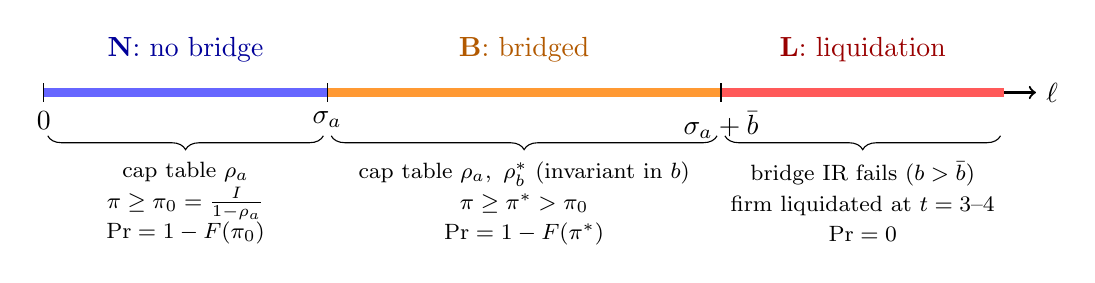
\begin{tikzpicture}[xscale=1.0, yscale=1.0]
% axis
\draw[->, thick] (0,0) -- (12.6,0) node[right] {$\ell$};
% segments
\draw[line width=3pt, blue!60]   (0,0) -- (3.6,0);
\draw[line width=3pt, orange!80] (3.6,0) -- (8.6,0);
\draw[line width=3pt, red!65]    (8.6,0) -- (12.2,0);
% ticks
\foreach \x/\lab in {0/$0$, 3.6/$\sigma_a$, 8.6/$\sigma_a+\bar b$}
  \draw (\x,0.12) -- (\x,-0.12) node[below] {\lab};
% region names
\node[blue!60!black]   at (1.8, 0.55) {\textbf{N}: no bridge};
\node[orange!70!black] at (6.1, 0.55) {\textbf{B}: bridged};
\node[red!60!black]    at (10.4,0.55) {\textbf{L}: liquidation};
% braces with conditional objects
\draw[decorate, decoration={brace, mirror, amplitude=5pt}] (0.05,-0.55) -- (3.55,-0.55)
  node[midway, below=6pt, align=center] {\footnotesize cap table $\rho_a$\\[-1pt]\footnotesize $\pi\ge\pi_0=\frac{I}{1-\rho_a}$\\[-1pt]\footnotesize $\Prob=1-F(\pi_0)$};
\draw[decorate, decoration={brace, mirror, amplitude=5pt}] (3.65,-0.55) -- (8.55,-0.55)
  node[midway, below=6pt, align=center] {\footnotesize cap table $\rho_a,\ \rho_b^{*}$ (invariant in $b$)\\[-1pt]\footnotesize $\pi\ge\pi^{*}>\pi_0$\\[-1pt]\footnotesize $\Prob=1-F(\pi^{*})$};
\draw[decorate, decoration={brace, mirror, amplitude=5pt}] (8.65,-0.55) -- (12.15,-0.55)
  node[midway, below=6pt, align=center] {\footnotesize bridge IR fails ($b>\bar b$)\\[-1pt]\footnotesize firm liquidated at $t=3$--$4$\\[-1pt]\footnotesize $\Prob=0$};
\end{tikzpicture}
\caption{Partition of the liquidity shock. The lower boundary is mechanical (the accelerator's cash); the upper boundary is endogenous (the bridge's participation cap \eqref{eq:cap}). Within each region the seed-stage cap table --- hence the financing threshold --- is constant; within B this constancy is exactly the share-invariance result of Corollary~\ref{cor:invariance}.}
\label{fig:partition}
\end{figure}

\paragraph{Assembling the identity.} Since $\pi$ and $\ell$ are independent, iterate expectations: condition on the region of $\ell$, then apply the region's conditional seed probability.

\begin{proposition}[Participation cap and the seed-probability decomposition]\label{prop:participation}
The bridge intervenes if and only if $b=\ell-\sigma_a \in (0, \bar b\,]$ with $\bar b$ given by \eqref{eq:cap}; letting $G$ denote the c.d.f.\ of $\ell$, the ex-ante probability of bridge intervention is $G(\sigma_a+\bar b)-G(\sigma_a)$. The ex-ante probability of a successful seed round is
\begin{equation}
\Prob(\text{seed})
\;=\;
\underbrace{G(\sigma_a)}_{\Prob(\mathrm{N})}\,\bigl[1-F(\pi_0)\bigr]
\;+\;
\underbrace{\bigl[G(\sigma_a+\bar b) - G(\sigma_a)\bigr]}_{\Prob(\mathrm{B})}\,\bigl[1-F(\pi^{*})\bigr]
\;+\;
\underbrace{\bigl[1-G(\sigma_a+\bar b)\bigr]}_{\Prob(\mathrm{L})}\cdot\, 0,
\label{eq:probseed}
\end{equation}
with $\pi_0 = I/(1-\rho_a) < \pi^{*} < 1$.
\end{proposition}

\begin{proof}
The regional decomposition and the constancy of the threshold within each region are established above; the only nontrivial ingredients are (i) share invariance, which delivers a single $\pi^{*}$ across B (Corollary~\ref{cor:invariance}), and (ii) $\pi_0<\pi^{*}$, i.e.\ bridge equity strictly crowds the cap table, proved in Proposition~\ref{prop:uniform} for the uniform benchmark ($g(\pi_0)<0$ places the root above $\pi_0$) and following in general from $\rho_b^{*}>0$ in \eqref{eq:threshold}. Independence of $\pi$ and $\ell$ then gives \eqref{eq:probseed} by the law of total probability.
\end{proof}

\begin{remark}[Why a single bridged threshold is not innocuous]
Absent share invariance, the bridged region would carry a threshold \emph{function} $\pi^{*}(b)$ and \eqref{eq:probseed} would read $\int_{\sigma_a}^{\sigma_a+\bar b}[1-F(\pi^{*}(\ell-\sigma_a))]\,\dd G(\ell)$ --- still computable, but no longer separating the shock distribution from the project-quality distribution. It is the monopolist bridge's share-targeting behavior that collapses the integral into the product $\Prob(\mathrm{B})\times[1-F(\pi^{*})]$; under alternative closures (competitive bridges, Section~\ref{sec:extensions}), and within the round-conversion regime of Proposition~\ref{prop:neutrality}(ii) where the threshold moves with $b$, the integral form returns.
\end{remark}

Equation \eqref{eq:probseed} is the model's central accounting identity, and every policy comparative static in the sequel operates through exactly one of two channels: \emph{moving mass across regions} (the boundaries $\sigma_a$ and $\sigma_a+\bar b$ shift --- the cash channel moves both one-for-one, the MFN moves the upper one through $\bar b$) or \emph{moving the thresholds within regions} ($\pi_0$ and $\pi^{*}$ respond to $\rho_a$, $I$, and the MFN tranche). Reading each policy through this two-channel lens is what keeps the reform analysis of Section~\ref{sec:reform} transparent.

\section{Uniform benchmark}\label{sec:uniform}

Let $f \equiv 1$ on $[0,1]$, so $M(x) = \tfrac{1-x^2}{2}$. Equation \eqref{eq:thresholdeq} becomes
\begin{equation}
(1-\rho_a)\,\pi^{3} \;=\; I\;\frac{1+\pi^{2}}{2}
\qquad\Longleftrightarrow\qquad
g(\pi) \;\equiv\; 2(1-\rho_a)\,\pi^{3} - I\,\pi^{2} - I \;=\; 0 .
\label{eq:cubic}
\end{equation}

\begin{proposition}[Existence, uniqueness, comparative statics]\label{prop:uniform}
Assume $I < 1-\rho_a$. Then \eqref{eq:cubic} has a unique root $\pi^{*} \in (0,1)$; it lies on the increasing branch of $g$ (so $g'(\pi^{*})>0$) and satisfies $\pi^{*} > \pi_0 = I/(1-\rho_a)$, ensuring $V_b^{*} > 0$. Moreover
\[
\frac{\dd \pi^{*}}{\dd \rho_a} \;=\; \frac{2\pi^{*3}}{g'(\pi^{*})} \;>\;0,
\qquad
\frac{\dd \pi^{*}}{\dd I} \;=\; \frac{1+\pi^{*2}}{g'(\pi^{*})} \;>\;0,
\]
and consequently $\rho_b^{*}$ and $\bar b$ are strictly decreasing in $\rho_a$, while $V_b^{*}$ is strictly increasing in $\rho_a$ (both directly and through $\pi^{*}$). If $I \ge 1-\rho_a$, no interior threshold exists: the project is unfinanceable at any bridge valuation.
\end{proposition}

\begin{proof}
$g(0) = -I <0$ and $g(1) = 2(1-\rho_a) - 2I > 0$ iff $I<1-\rho_a$. Since $g'(\pi) = 2\pi\bigl[3(1-\rho_a)\pi - I\bigr]$, $g$ decreases then increases on $(0,1)$ with trough at $I/[3(1-\rho_a)]<\tfrac13$; as $g(0)<0$, the root is unique and lies on the increasing branch. At $\pi_0$, $g(\pi_0) = 2I\pi_0^2 - I\pi_0^2 - I = I(\pi_0^{2}-1)<0$, hence $\pi^{*}>\pi_0$ and $1-\rho_a-I/\pi^{*}>0$. The derivatives follow from the implicit function theorem with $\partial g/\partial \rho_a = -2\pi^{3}$ and $\partial g/\partial I = -(1+\pi^{2})$. For $\rho_b^{*} = 1-\rho_a - I/\pi^{*}$: $\dd\rho_b^{*}/\dd\rho_a = -1 + (I/\pi^{*2})(\dd\pi^{*}/\dd\rho_a) = -1 + I\big/[3(1-\rho_a)\pi^{*}-I]$, negative iff $3(1-\rho_a)\pi^{*} > 2I$, which holds since $\pi^{*}>\pi_0 = I/(1-\rho_a) > 2I/[3(1-\rho_a)]$. Then $\bar b = M(\pi^{*})\rho_b^{*}$ falls in $\rho_a$ as the product of two positive decreasing terms, and $V_b^{*} = b/\rho_b^{*}$ rises.
\end{proof}

The condition $I < 1-\rho_a$ reads directly: the investment cost must not exceed the equity left over by the accelerator, otherwise even a maximally generous bridge cannot make the seed round feasible for any $\pi \le 1$.

\begin{remark}[Certainty equivalence and Jensen's inequality]\label{rem:jensen}
If the bridge must choose $V_b$ before $I$ is revealed (holding a prior over $I$), replacing $I$ by $\E(I)$ in \eqref{eq:cubic} is only a certainty-equivalent approximation. Since $\pimin(I) = V_b I/[(1-\rho_a)V_b - I]$ is strictly convex in $I$ on its admissible range, $\E[\pimin(I)] > \pimin(\E I)$: the certainty-equivalent calculation \emph{understates} the average threshold, the more so the larger $\operatorname{Var}(I)$ and the closer $\E(I)$ to the feasibility frontier. The exact ex-ante first-order condition is the $I$-weighted average of \eqref{eq:FOC}; see Section~\ref{sec:extensions}.
\end{remark}

\section{The 2022 reform}\label{sec:reform}

The reform changes the accelerator's proposal from $(\$125\text{K}, 7\%)$ to $\bigl(\$500\text{K},\, 7\% + \$375\text{K}/\min\{V, V_b\}\bigr)$. It bundles two instruments that the model cleanly separates.

\paragraph{Benchmark calibration.} Numerical statements throughout refer to the uniform$\times$uniform benchmark: terminal values normalized so that the support of $\pi$ is $[0,1]$ with unit ``\$30M''; $I=\$2\text{M}=0.067$; $\ell\sim U[0,\,\$1.5\text{M}]$ ($L=0.05$); headline stake $\rho_a^{0}=7\%$; and the two observed deals $\sigma_a=\$125$K (old) and $\sigma_a=\$500$K with $m=\$375$K (new). At these parameters: $\pi_0=0.072$ (old deal), $\pi^{*}=0.342$ (the bridged threshold, written $\pi_1$ from Section~\\ref{sec:mfnchannel} on), $\rho_b^{\mathrm{tot}}=0.735$, and $\bar b=\$9.7$M $\gg L$ --- the participation cap is slack, so the post-reform drop in bridge incidence below is a pure cash effect.

\subsection{Cash channel: $\sigma_a \uparrow$}

Raising $\sigma_a$ leaves $\pi_0$, $\pi^{*}$, $\rho_b^{*}$, and $\bar b$ unchanged (Corollary~\ref{cor:invariance}) but shifts the shock partition in \eqref{eq:probseed}: the no-bridge region $\{\ell \le \sigma_a\}$ expands, the liquidation region $\{\ell > \sigma_a + \bar b\}$ recedes. Since $\pi_0 < \pi^{*}$, mass moves from the bridged region (success probability $1-F(\pi^{*})$) and the liquidation region (success probability $0$) into the no-bridge region (success probability $1-F(\pi_0)$):
\[
\frac{\partial \Prob(\text{seed})}{\partial \sigma_a}
= g_\ell(\sigma_a)\bigl[F(\pi^{*})-F(\pi_0)\bigr]
+ g_\ell(\sigma_a+\bar b)\bigl[1-F(\pi^{*})\bigr] \;>\;0,
\]
where $g_\ell$ is the density of $\ell$. The cash channel unambiguously raises seed success and unambiguously lowers the probability that a bridge is needed at all.

\subsection{The bridge's optimal contract, and the SAFE's ratchet}\label{sec:safebridge}

The benchmark endowed the bridge with a \emph{priced} instrument. Before adding YC's tranche, ask the prior question: if the bridge could sign \emph{any} conversion rule --- a fixed share, a capped SAFE, a discount, a schedule contingent on the round --- which would it choose? The answer is clean, because the seed stage compresses every instrument to a single degree of freedom.

\paragraph{One degree of freedom.} Let the bridge's claim assign it a share $s(V)$, possibly contingent on the round valuation. At $t=7$ the seed's cap-table constraint binds, $\rho_s=k-s(V)$ with $k\equiv1-\rho_a$, and the round prices at $V=I/\rho_s$; the seed finances iff $\pi\ge V$. Whatever the rule, the equilibrium therefore delivers a single pair --- a realized share $s$ and a threshold $\pimin=V$ --- linked by
\[
s \;=\; k-\frac{I}{\pimin}.
\]
The bridge's payoff is $s\,M(\pimin)-b=\varphi_I(\pimin)-b$, where $\varphi_I(\pi)\equiv(k-I/\pi)M(\pi)$ is the overhang value at threshold $\pi$: \emph{choosing an instrument is choosing a point on the overhang-value hill}, nothing more.

\paragraph{The SAFE's reach.}
The standard instrument does not offer a free choice on that hill. A SAFE with cap $V_b$ converts at the \emph{better} of the cap and the round price --- the cap is investor protection, an embedded full ratchet, not a firm price.\footnote{Y Combinator's primer for the post-money safe is explicit: when the round valuation does not sufficiently exceed the cap, the safe holder receives shares at the price paid by the new-money investors; the original safe already operated this way. The exact crossover involves post-money capitalization mechanics; at the model's resolution, conversion at $\min\{V_b, V\}$ is the right stylization.} Which thresholds can the bridge then induce? Solve the seed-stage fixed point for each $V_b$, in two cases.

\emph{Case 1: the cap binds ($V_b\le V$).} The SAFE converts at $V_b$, the bridge holds $b/V_b$, and the seed's saturated cap table gives
\[
\rho_a+\frac{b}{V_b}+\frac{I}{V}=1
\quad\Longrightarrow\quad
\pimin=V=\frac{I}{\,k-b/V_b\,}.
\]
The conjecture $V_b\le V$ rearranges to $kV_b-b\le I$, i.e.\ $V_b\le\hat V_0(b)\equiv\tfrac{I+b}{k}$. On this segment the mechanics run through the seed's residual: the cap is the price per unit of equity the bridge pays, so raising it buys \emph{fewer} shares for the same check $b$, leaves more equity to the seed, and \emph{lowers} the threshold $I/(k-b/V_b)$ --- a high cap is the bridge's gift to the financing chain --- down to $\pimin(\hat V_0)=\hat V_0$ exactly at the kink. Lowering the cap does the opposite, until at the floor $V_b\downarrow b/k$ the bridge's share exhausts the available cap table, nothing remains for the seed, and the threshold diverges. The map $V_b\mapsto\pimin$ is thus a continuous decreasing bijection from $(b/k,\,\hat V_0]$ onto $[\hat V_0(b),\,+\infty)$: Case 1 generates every threshold in that range, each through exactly one cap.

\emph{Case 2: the round prices below the cap ($V_b>\hat V_0(b)$).} The ratchet fires: the SAFE converts at the round, the bridge holds $b/V$, and the cap table gives
\[
\rho_a+\frac{b+I}{V}=1
\quad\Longrightarrow\quad
V=\frac{I+b}{k}=\hat V_0(b)
\quad\text{\emph{regardless of} } V_b .
\]
The written cap has dropped out of every equation: the threshold is $\hat V_0(b)$ and the bridge's payoff is flat in $V_b$.

Combining the cases, the SAFE's attainable thresholds are exactly $[\hat V_0(b),+\infty)$: \emph{the ratchet walls off every threshold below $\hat V_0(b)$}. The chain that builds the wall is worth spelling out: a low threshold requires a small bridge share; a small share requires a high conversion price; and the SAFE cannot commit to a high price --- as soon as the cap exceeds $\hat V_0$, the round prices below it and the ratchet automatically hands the bridge the round price, hence the larger share $b/\hat V_0$. The bridge cannot refuse its own protection; it is wired into the instrument. The smallest share a SAFE can deliver is $b/\hat V_0(b)$, full stop --- whereas a priced instrument can promise any share, including one \emph{smaller than new money gets per dollar}, and that committed generosity is what keeps the cap table light.\footnote{At the benchmark with $b=0.28$: $\hat V_0=0.373$, walling off the target $\pi^{*}=0.342$. The priced instrument reaches it at $V_b=b/(k-I/\pi^{*})=0.381$ --- a conversion price \emph{above} the round's $0.342$, i.e.\ fewer shares per dollar than the seed receives, which no SAFE would ever concede to itself.}

\paragraph{Regularity from log-concavity.}
Before characterizing either instrument's optimum, settle two questions once and for all --- whether first-order conditions pin unique thresholds, and whether profits are single-peaked --- from a single shape restriction on the primitive. The results are stated for a general cost parameter $J$ (here $J=I$; the MFN tranche below uses the same family), through the family
\begin{equation}
A(\pi, J)\;\equiv\; k\,\pi^{3}f(\pi)\;-\;J\,\pi^{2}f(\pi)\;-\;J\,M(\pi).
\label{eq:Afamily}
\end{equation}

\begin{assumption}[LC]\label{ass:LC}
$f$ is log-concave on $(0,1)$.
\end{assumption}

This is the workhorse class of information economics --- it contains the uniform, Beta$(\alpha,\beta)$ with $\alpha,\beta\ge1$, truncated normal, logistic, and exponential densities, among many others (Bagnoli and Bergstrom, 2005) --- and it is the \emph{only} shape assumption of this section.

\begin{lemma}[Value-weighted hazard]\label{lem:hazard}
Let $\lambda(\pi)\equiv\dfrac{\pi f(\pi)}{M(\pi)}$, the hazard rate of the value-weighted project distribution (density $u f(u)/\E(\pi)$ on $(0,1)$). Under (LC), $\lambda$ is nondecreasing, and $\pi\mapsto\pi\lambda(\pi)$ is strictly increasing, with $\pi\lambda(\pi)\to0$ as $\pi\to0^{+}$ and $\pi\lambda(\pi)\to+\infty$ as $\pi\to1^{-}$.
\end{lemma}

\begin{proof}
$\log\bigl(uf(u)\bigr)=\log u+\log f(u)$ is a sum of concave functions, so the tilted density $g(u)\equiv uf(u)$ is log-concave; a log-concave density has nondecreasing hazard rate (Bagnoli and Bergstrom, 2005, Theorem 1), i.e.\ $\lambda=g/M$ is nondecreasing. Strict monotonicity of $\pi\lambda(\pi)$ then comes for free from the strictly increasing factor $\pi$. Endpoints: near $0$, $f$ is bounded (a concave $\log f$ cannot tend to $+\infty$ at the boundary of an open interval), so $\pi\lambda=\pi^{2}f/M\to0$. Near $1$, write $g=e^{\varphi}$ with $\varphi$ concave; where $\varphi'(\pi)\le0$ the tangent bound $g(u)\le g(\pi)e^{\varphi'(\pi)(u-\pi)}$ gives $M(\pi)=\int_\pi^1 g\le g(\pi)(1-\pi)$, hence $\lambda(\pi)\ge1/(1-\pi)\to\infty$; if instead $g$ increases up to $1$, then $g(1)>0$ and $M(\pi)\sim g(1)(1-\pi)$ gives the same conclusion.
\end{proof}

\begin{lemma}[The $\Psi$ curve]\label{lem:psi}
Define
\[
\Psi(\pi)\;\equiv\;\frac{k\,\pi^{3}f(\pi)}{\pi^{2}f(\pi)+M(\pi)}
\;=\;\frac{k\pi}{1+\dfrac{1}{\pi\lambda(\pi)}}.
\]
Then the family \eqref{eq:Afamily} factorizes as
\[
A(\pi,J)\;=\;\bigl(\pi^{2}f(\pi)+M(\pi)\bigr)\,\bigl[\Psi(\pi)-J\bigr],
\]
with a strictly positive first factor; and under (LC), $\Psi$ is strictly increasing on $(0,1)$, mapping it onto $(0,k)$.
\end{lemma}

\begin{proof}
The factorization is immediate. Monotonicity: $\pi\lambda(\pi)$ is strictly increasing (Lemma~\ref{lem:hazard}) and $x\mapsto1/(1+1/x)$ is increasing, so $\Psi$ is a product of two strictly/weakly increasing positive factors, strictly increasing overall through the factor $k\pi$. Endpoints: $\pi\lambda\to0$ gives $\Psi\to0$; $\pi\lambda\to\infty$ gives $\Psi\to k$.
\end{proof}

The bridge's first-order condition on either branch now reads $\Psi(\pi)=J$: $\Psi(\pi)$ is \emph{the investment cost that rationalizes threshold $\pi$}, and the shape restriction of the model is the increasing-hazard condition familiar from the rest of information economics, applied here to the value-weighted project distribution.

\begin{corollary}[Regularity]\label{lem:regularity}
Under (LC), for any cost parameter $J<k$:
\begin{enumerate}[label=(\alph*), itemsep=0pt]
\item for each $J\in\{I,\,I+m\}$, $A(\cdot,J)$ has the \emph{unique} root $\pi(J)=\Psi^{-1}(J)$, with $A<0$ below it and $A>0$ above; existence of the root is \emph{equivalent} to $J<k$ --- the maintained admissibility $I<1-\rho_a$ for $J=I$, and Assumption~(F) below for $J=I+m$;
\item $\pi(J)$ is strictly increasing in $J$ and in $\rho_a^{0}$; in particular $\pi_1\equiv\pi(I)<\pi(I+m)\equiv\pi_2$;
\item on each branch, $\Pi_b$ is single-peaked in $V_b$: strictly increasing below its first-order-condition point and strictly decreasing above.
\end{enumerate}
\end{corollary}

\begin{proof}
(a)--(b): monotone inversion of $\Psi$; the range $(0,k)$ makes existence equivalent to $J<k$; and $\Psi$ is proportional to $k=1-\rho_a^{0}$, so lowering $k$ raises $\Psi^{-1}(J)$. (c): by \eqref{eq:profitA} and the factorization, $\operatorname{sign}\Pi_b'(V_b)=\operatorname{sign}\bigl(\Psi(\pimin(V_b))-J\bigr)$; since $\pimin(\cdot)$ is strictly decreasing, $V_b$ below the FOC point means $\pimin$ above $\pi(J)$, where $\Psi>J$, and conversely.
\end{proof}




\paragraph{The proposition.}

\begin{proposition}[The bridge's optimal contract]\label{prop:instrument}
Under (LC):
\begin{enumerate}[label=(\roman*), itemsep=0pt]
\item Over all conversion rules, the bridge's maximal payoff is $\Pi^{\mathrm{opt}}(b)=\varphi_I(\pi^{*})-b$, the peak of the overhang-value hill; it is implemented by a \emph{priced} instrument --- the fixed share $\rho_b^{*}=k-I/\pi^{*}$ --- for every need $b$.
\item A capped SAFE implements the optimum if and only if $b\le T_1^{0}\equiv k\pi^{*}-I$ (the \emph{latent} region, where its equilibrium cap satisfies $V_b^{*}\le V$ and the ratchet never fires). Beyond it, the SAFE's payoff is $\varphi_I(\hat V_0(b))-b<\Pi^{\mathrm{opt}}(b)$: \emph{the ratchet strictly hurts its holder}.
\item Participation caps order accordingly: $\bar b^{\mathrm{priced}}=\varphi_I(\pi^{*})=M(\pi^{*})\rho_b^{*}$, while $\bar b^{\mathrm{SAFE}}=k\bar x-I\le\bar b^{\mathrm{priced}}$ whenever $\pi^{*}<\bar x$ (and the caps coincide otherwise), where $\bar x$ solves $M(\bar x)=\bar x$.
\end{enumerate}
\end{proposition}

\begin{proof}
(i) By the one-degree-of-freedom reduction, any rule's payoff is $\varphi_I(\pimin)-b$; a fixed share $\rho_b$ implements any threshold $\pimin=I/(k-\rho_b)$ in $(I/k,\,1)$; and $\varphi_I$ is strictly quasiconcave with interior peak $\pi^{*}=\Psi^{-1}(I)$ by the factorization of Lemma~\ref{lem:psi} at $J=I$. (ii) The SAFE's attainable set is $[\hat V_0(b),\infty)$; it contains $\pi^{*}$ iff $\pi^{*}\ge\hat V_0(b)$ iff $b\le T_1^{0}$; beyond, the best attainable threshold is $\hat V_0(b)$ (the branch increases up to the kink by Corollary~\ref{lem:regularity}(c), and is flat past it), and $\varphi_I(\hat V_0(b))<\varphi_I(\pi^{*})$ by strict quasiconcavity since $\hat V_0(b)>\pi^{*}$. (iii) $\varphi_I(\pi^{*})\ge b$ gives the priced cap; the SAFE's value beyond $T_1^{0}$ is nonnegative iff $M(\hat V_0)\ge\hat V_0$, i.e.\ $b\le k\bar x-I$; and $\varphi_I(\pi^{*})\ge\varphi_I(\bar x)=k\bar x-I$ by optimality of $\pi^{*}$. When $\pi^{*}\ge\bar x$ the SAFE frontier falls in the latent region and the caps coincide.
\end{proof}

The economics deserves a sentence, because it runs against instinct: the ratchet is a \emph{protection}, yet it hurts. By guaranteeing the bridge the round price whenever the round prices low, the ratchet mechanically loads the cap table in exactly those states, raises the financing threshold, and destroys the conversion states the bridge's claim pays in --- the protection turns against its holder through the cap-table externality. The priced instrument is a \emph{commitment device}: ``I will not ratchet,'' which leaves the seed room. Two empirical echoes: distressed bridges should be \emph{priced} rounds (they are: down rounds in distress are priced); and the overwhelming dominance of SAFEs in practice --- $90\%$ of pre-seed rounds --- reads, through the proposition, as the market revealing that typical needs live in the latent region $b\le T_1^{0}$, where the instruments coincide and the SAFE wins on transaction costs.

\subsection{MFN channel: the tranche meets the ratchet}\label{sec:mfnchannel}

With the MFN tranche $m=\$375$K, the accelerator's effective share in the bridge state is
\begin{equation}
\rho_a^{\mathrm{eff}} \;=\; \rho_a^{0} + \frac{m}{\min\{V, V_b\}},
\label{eq:rhoeff}
\end{equation}
the tranche converting at the lowest cap issued before the round, or at the round price if that is lower still. From here on $k\equiv1-\rho_a^{0}$. The analysis layers the tranche on the SAFE bridge of Section~\ref{sec:safebridge}; the fixed-point construction is identical with $b+m$ of convertible money in the low-cap regime and $I+m+b$ at the kink.

\paragraph{Feasibility.}

\begin{assumption}[F]\label{ass:F}
$I+m < 1-\rho_a^{0}$.
\end{assumption}

\begin{lemma}[Infeasibility otherwise]\label{lem:infeasible}
If $I+m\ge k$, no state is financeable: the no-bridge threshold $(I+m)/k$ and the bridged thresholds (both $I/(k-\tfrac{b+m}{V_b})$ below the kink and $\hat V(b)$ at and beyond it) all exceed $1$, and the bridge never participates.
\end{lemma}

\begin{proof}
Below: $\pimin\ge\pimin(\hat V)=\hat V=(I+m+b)/k\ge(I+m)/k\ge1$ by monotonicity; at and beyond the kink the threshold is $\hat V\ge1$; in the no-bridge states the tranche converts at the round and $\pi_0=(I+m)/k\ge1$.
\end{proof}

Assumption~(F) generalizes the Game-1 condition $I<1-\rho_a$ and reads as a \emph{cap on the tranche}: $m<k-I$.

\paragraph{The conversion fixed point with the tranche.}

\begin{lemma}[Conversion fixed point and kink]\label{lem:kink}
For every $V_b$ the seed-stage fixed point is unique and switches at
\[
\hat V(b)\;\equiv\;\frac{I+m+b}{k}:
\]
for $V_b\le\hat V(b)$, the bridge SAFE carries the lowest cap, the tranche and the bridge convert at $V_b$, and $\pimin=I\big/\bigl(k-\tfrac{b+m}{V_b}\bigr)$; for $V_b>\hat V(b)$, \emph{everything} converts at the round price, $V=\hat V(b)$ identically, and the bridge's profit is flat in $V_b$. In both regimes the seed finances iff $\pi\ge V$, so $\pimin=V$, continuous at the kink with $\pimin(\hat V)=\hat V$.
\end{lemma}

\begin{proof}
Conjecture conversion at $V_b$: the seed constraint binds, $\rho_s=k-(b+m)/V_b$, $V=I/\rho_s$; consistency $V_b\le V$ holds iff $V_b\le\hat V$. Conjecture conversion at the round: the constraint binds at $\rho_a^{0}+(m+b+I)/V=1$, so $V=\hat V(b)$ regardless of $V_b$; consistency $V<V_b$ iff $V_b>\hat V$. Flatness: in the latter regime neither shares nor threshold depend on $V_b$. The participation of the seed, $(I/V)\pi-I\ge0$, reads $\pi\ge V$ in both regimes.
\end{proof}

\paragraph{The low-cap branch.}
On $V_b\le\hat V(b)$ the bridge's objective is $\Pi_b(V_b)=b\,[M(\pimin)/V_b-1]$ with
\[
\pimin=\frac{I}{k-\frac{b+m}{V_b}},
\qquad
\frac{\partial\pimin}{\partial V_b}=-\frac{\pimin^{2}}{I}\cdot\frac{b+m}{V_b^{2}}<0 .
\]
Differentiating, with $M'=-\pimin f(\pimin)$ (Leibniz):
\[
\Pi_b'(V_b)
= b\left[\frac{M'(\pimin)\,\partial_{V_b}\pimin}{V_b}-\frac{M(\pimin)}{V_b^{2}}\right]
= \frac{b}{V_b^{2}}\left[\frac{(b+m)\,f(\pimin)\,\pimin^{3}}{I\,V_b}-M(\pimin)\right].
\]
Along the branch the identity $\tfrac{b+m}{V_b}=k-\tfrac{I}{\pimin}$ holds by construction; substituting it collapses the bracket into the family \eqref{eq:Afamily} of Section~\ref{sec:safebridge}:
\begin{equation}
\Pi_b'(V_b)\;=\;\frac{b}{V_b^{2}}\cdot\frac{A\bigl(\pimin(V_b),\,I\bigr)}{I}:
\label{eq:profitA}
\end{equation}
the branch first-order condition is the Game-1 threshold equation \eqref{eq:thresholdeq} at the headline stake --- the tranche has vanished from it, a first glimpse of neutrality.

\paragraph{The dichotomy.}
The branch first-order condition targets the threshold $\pi_1\equiv\pi(I)=\Psi^{-1}(I)$, a horizontal level independent of $b$ (share invariance again), while the branch's reach is $[\hat V(b),\infty)$ with $\hat V(b)$ an increasing line. The candidate is attainable iff
\[
\pi_1\;\ge\;\hat V(b)
\quad\Longleftrightarrow\quad
b\;\le\;T_1\;\equiv\;k\,\pi_1-(I+m),
\]
the crossing point of level and line (Figure~\ref{fig:regimes}). Beyond it, the branch is increasing throughout (Corollary~\ref{lem:regularity}(c)) and the profit is flat past the kink: the outcome is conversion at the round.

\begin{figure}[t]
\centering
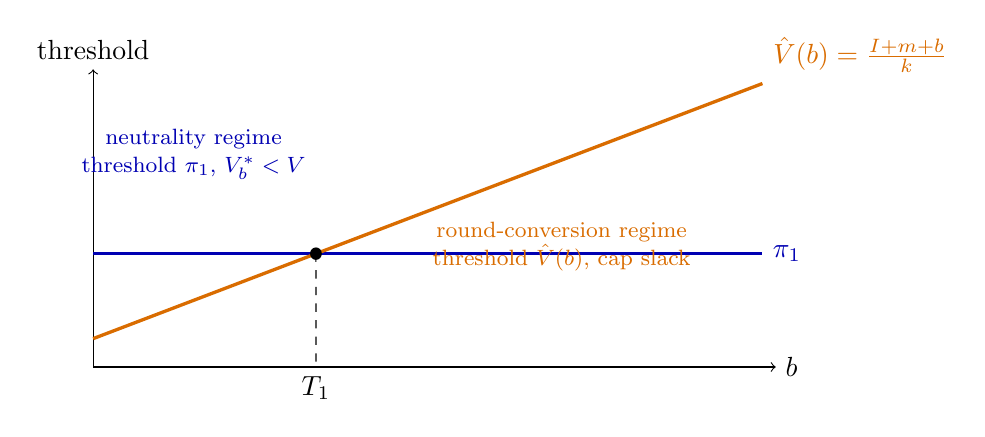
\begin{tikzpicture}[xscale=8.5, yscale=9.0]
\draw[->] (0,0.30) -- (1.02,0.30) node[right] {$b$};
\draw[->] (0,0.30) -- (0,0.72) node[above] {threshold};
\draw[blue!70!black, thick] (0,0.46) -- (1.0,0.46) node[right] {$\pi_1$};
\draw[orange!85!black, very thick] (0,0.34) -- (1.0,0.70) node[above right] {$\hat V(b)=\frac{I+m+b}{k}$};
\coordinate (A) at (0.333,0.46);
\draw[dashed] (A) -- (0.333,0.30) node[below] {$T_1$};
\fill (A) circle (0.25pt);
\node[align=center, blue!70!black]  at (0.15,0.60) {\footnotesize neutrality regime\\[-2pt]\footnotesize threshold $\pi_1$, $V_b^{*}<V$};
\node[align=center, orange!85!black] at (0.70,0.47) {\footnotesize round-conversion regime\\[-2pt]\footnotesize threshold $\hat V(b)$, cap slack};
\end{tikzpicture}
\caption{The dichotomy as a crossing problem. The low-cap branch's first-order condition pins the horizontal level $\pi_1$ (independent of $b$); the conversion kink $\hat V(b)$ is an increasing line. Left of the crossing $T_1$, the candidate is attainable and the MFN is threshold-neutral; right of it, every convertible converts at the round price and the written cap is slack.}
\label{fig:regimes}
\end{figure}

\paragraph{The proposition, on general $f$.}

\begin{proposition}[MFN under the SAFE bridge: neutrality and round conversion]\label{prop:neutrality}
Under (F) and (LC), the bridge state resolves into two regimes:
\begin{enumerate}[label=(\roman*), itemsep=0pt]
\item \textbf{Small needs ($b\le T_1$): neutrality and repricing.} The threshold is $\pi_1$ --- the Game-1 equation at the \emph{headline} stake and cost $I$, independent of $m$ --- and
\[
V_b^{*} \;=\; \frac{b+m}{\rho_b^{\mathrm{tot}}} \;\le\; \hat V(b)\;\le\; \pi_1=V,
\qquad
\rho_b^{\mathrm{tot}}\equiv k-\frac{I}{\pi_1},
\qquad
\frac{b}{V_b^{*}} = \rho_b^{\mathrm{tot}}\frac{b}{b+m},
\quad
\frac{m}{V_b^{*}} = \rho_b^{\mathrm{tot}}\frac{m}{b+m}:
\]
the valuation rises by the uplift $(b+m)/b$ and the unchanged total convertible share is split pro rata to cash. The MFN leaves the bridged threshold, and the conditional seed probability, untouched.
\item \textbf{Large needs ($b>T_1$): conversion at the round.} Every convertible converts at $V=\hat V(b)=(I+m+b)/k$; the threshold is $\hat V(b)$, strictly increasing in the need; the written cap is payoff-irrelevant on $[\hat V,\infty)$ --- equivalently, the bridge might as well go uncapped. Empirical implication: beyond the neutrality region, bridge SAFEs' effective conversion price equals the round price --- caps slack or absent.
\item \textbf{Participation.} Let $\bar x$ solve $M(\bar x)=\bar x$. The frontier falls in regime (i) or (ii) according to the dichotomy
\[
\bar b_{\mathrm{MFN}} \;=\;
\begin{cases}
M(\pi_1)\,\rho_b^{\mathrm{tot}}-m & \text{if } \pi_1\ge\bar x \quad(\text{frontier in (i)}),\\[2pt]
k\,\bar x-(I+m) & \text{if } \pi_1<\bar x \quad(\text{frontier in (ii)}).
\end{cases}
\]
Relative to the SAFE bridge without the tranche (Section~\ref{sec:safebridge}), the cap shrinks by \emph{exactly} $m$ in the second case, and by exactly $m$ in the first as well: against the correct benchmark, the tranche crowds out one dollar of bridge capacity per dollar of tranche.
\item \textbf{No-bridge states.} When $\ell\le\sigma_a$, the tranche converts at the round and $\pi_0=(I+m)/k$: the MFN taxes the investment cost by $m$.
\end{enumerate}
\end{proposition}

\begin{proof}
(i): the branch FOC point solves $A(\pi,I)=0$, attainable iff $b\le T_1$; the valuation inverts the branch identity $\tfrac{b+m}{V_b}=k-\tfrac{I}{\pi_1}$, and the chain $V_b^{*}\le\hat V(b)\le\pi_1=V$ holds since $b\le T_1$. (ii): beyond $T_1$, the branch is increasing up to the kink by Corollary~\ref{lem:regularity}(c) (its FOC point is out of reach) and Lemma~\ref{lem:kink} makes the profit flat past it: any $V_b\ge\hat V$ is optimal, with threshold $\hat V(b)$. (iii): regime-(i) profit is nonnegative iff $b+m\le M(\pi_1)\rho_b^{\mathrm{tot}}$; this frontier lies within $[0,T_1]$ iff $M(\pi_1)\le\pi_1$, i.e.\ $\pi_1\ge\bar x$. Regime-(ii) profit is $b\,[M(\hat V)/\hat V-1]\ge0$ iff $\hat V\le\bar x$, i.e.\ $b\le k\bar x-(I+m)$; this frontier lies beyond $T_1$ iff $\pi_1<\bar x$. Exclusivity and exhaustiveness follow from the monotonicity of $M(x)-x$. Comparison with $m=0$: the Section-\ref{sec:safebridge} caps are $M(\pi^{*})\rho_b^{*}$ and $k\bar x-I$; in the second case the difference is exactly $m$; in the first, note $\pi_1$ and $\rho_b^{\mathrm{tot}}$ are the $m$-free Game-1 objects, so the cap is the $m=0$ cap minus $m$. (iv): the seed constraint binds at $\rho_a^{0}+m/V+I/V=1$.
\end{proof}

\begin{corollary}[The uniform benchmark]\label{cor:uniformOK}
$f\equiv1$ is log-concave, so Corollary~\ref{lem:regularity} applies; explicitly, $\Psi(\pi)=\dfrac{2k\pi^{3}}{1+\pi^{2}}$ and $\Psi(\pi)=J$ is, after clearing the denominator, the cubic $2k\pi^{3}-J\pi^{2}-J=0$ of Proposition~\ref{prop:uniform}. At the benchmark calibration: $\pi_1=0.342<\bar x=\sqrt2-1=0.414$, so the participation frontier falls in the round-conversion regime, $\bar b_{\mathrm{MFN}}=k\bar x-(I+m)=0.306$; the neutrality region ends at $T_1=0.239$ (a residual need of \$7.2M on the \$30M scale); and a direct numerical scan of the kinked profit function confirms the two regimes, the flatness beyond the kink, and the frontier at $0.306$.
\end{corollary}

\paragraph{The MFN under the bridge's optimal contract.} Proposition~\ref{prop:neutrality} takes the standard SAFE as the bridge's instrument. Section~\ref{sec:safebridge} says the bridge may prefer otherwise --- and the institutional detail cooperates: a priced bridge round is a bona fide Equity Financing, so it \emph{triggers the conversion of the accelerator's SAFEs at the bridge round itself}.\footnote{The safe converts at the first Equity Financing --- a bona fide transaction issuing preferred stock at a fixed valuation --- which a priced bridge round satisfies. The tranche then converts at $V_b$ for every $b$, and no round-price cap ever binds, since conversion precedes the seed round.} The tranche then converts at $V_b$ unconditionally, the kink disappears, and the low-cap-branch analysis applies for \emph{every} need:

\begin{corollary}[Global neutrality under the priced bridge]\label{cor:pricedmfn}
If the bridge finances through a priced round, the bridged threshold is $\pi_1$ for all $b$, the participation cap is $\bar b=M(\pi_1)\rho_b^{\mathrm{tot}}-m$, and the bridge weakly prefers this arrangement to the SAFE for every $b$ --- strictly on $b>T_1$ (its payoff is $\tfrac{b}{b+m}\,\varphi_I(\pi_1)-b$ against $\tfrac{b}{b+m}\,\varphi_I(\max\{\pi_1,\hat V(b)\})-b$). With free instrument choice, the round-conversion regime of Proposition~\ref{prop:neutrality}(ii) is therefore \emph{off the equilibrium path}: neutrality is global, and the dichotomy describes the world where the bridge is confined to the standard SAFE template. Reality sits in between, held to the SAFE by transaction costs exactly where the instruments coincide.
\end{corollary}

At the benchmark, the free-choice cap is $M(\pi_1)\rho_b^{\mathrm{tot}}-m=0.312$ against the SAFE-template cap $k\bar x-(I+m)=0.306$; a numerical scan of both instrument problems confirms the corollary's comparison at every $b$.

The economics: the neutrality of regime (i) is the share-targeting logic of Corollary~\ref{cor:invariance} pushed one step further --- the bridge targets the total convertible overhang and raises its valuation until the accelerator's conversion plus its own stake fill exactly that target, so the MFN's incidence falls on the bridge, not on the financing chain. But repricing needs \emph{room}: the conversion price of every claim is capped at the round price, and once the required valuation would exceed the round's, all claims convert at the round and the tranche degenerates into a tax of $m$ on the investment cost --- exactly as in the no-bridge states. \emph{Neutrality holds exactly as far as the bridge's repricing margin reaches, and no further.} (A priced bridge under the MFN would keep an interior problem beyond $T_1$ --- the Game-1 problem at cost $I+m$ --- but Proposition~\ref{prop:instrument}'s logic extends: the bridge itself weakly prefers the arrangement that keeps thresholds low.)

\begin{remark}[Where the calibration sits]\label{rem:calibrationregime}
At the benchmark, the liquidity-shock support keeps all bridged states deep inside the neutrality regime: residual needs satisfy $b\le L-\sigma_a=0.033$, an order of magnitude below $T_1=0.239$. The benchmark reform comparisons of this section are therefore unaffected by the regime structure; the round-conversion regime becomes quantitatively relevant only for distressed bridges --- needs of the order of the overhang value itself.
\end{remark}

\subsection{Net effect and testable predictions}

Combining channels, the reform's predictions are:

\begin{hypothesis}\label{hyp:pressure}
\textbf{(Ralston (i): fundraising pressure.)} Bridge incidence falls after the reform, through both channels: fewer companies need a bridge ($\sigma_a\uparrow$ expands the no-bridge region $\{\ell\le\sigma_a\}$) and the participation cap shrinks by \emph{exactly} $m$ against the SAFE-bridge benchmark (Proposition~\ref{prop:neutrality}(iii)). Conditional on a bridge occurring in the neutrality regime, valuations are higher by the closed-form uplift $(b+m)/b$ while the bridge's \emph{ownership stake} falls to $\rho_b^{\mathrm{tot}}\,b/(b+m)$; beyond it, effective conversion prices equal the round price --- written caps slack or absent. ``Less pressure to accept unfavorable terms'' maps to higher $V_b$ and lower bridge incidence --- with the sharp additional predictions that post-reform bridge valuations should rise roughly one-for-one with the \$375K tranche at given cash need, and that larger bridges should show slack or absent caps (and, by Proposition~\ref{prop:instrument} and Corollary~\ref{cor:pricedmfn}, migrate to priced rounds in distress --- where neutrality is restored and the tranche converts at the bridge round).
\end{hypothesis}

\begin{hypothesis}\label{hyp:founders}
\textbf{(Ralston (ii): founder participation.)} Not evaluable under the full-extraction closure (Remark~\ref{rem:fullext}): the entrepreneur's ex-ante equity value is zero in both games. Assessing whether the reform attracts more applicants requires a closure with positive founder rents --- e.g.\ a competitive seed stage --- under which the founder's ex-ante value inherits the reform's two channels with the same tension as below.
\end{hypothesis}

\begin{hypothesis}\label{hyp:seed}
\textbf{(Ralston (iii): seed success.)} Ambiguous, hence testable. By Proposition~\ref{prop:neutrality}, the decomposition is exact but the bridged region now subdivides: the cash channel raises $\Prob(\text{seed})$ (mass shifts to the no-bridge region, whose threshold is lowest); the MFN leaves the bridged threshold at $\pi_1$ on small needs and raises it to $\hat V(b)$ in the round-conversion regime --- where the identity gains an integral term $\int_{T_1}^{\bar b_{\mathrm{MFN}}}[1-F(\hat V(b))]\,\dd G(\sigma_a+b)$, the phenomenon anticipated by the remark of Section~\ref{sec:partition}; it also shrinks the bridged region at the top ($\bar b_{\mathrm{MFN}}<\bar b$) and raises the no-bridge threshold from $I/(1-\rho_a^0)$ to $(I+m)/(1-\rho_a^0)$. At the benchmark calibration the shock support keeps all bridged states in the small-needs regime (Remark~\ref{rem:calibrationregime}), so the simple two-region comparison applies; the sub-partition matters for calibrations with larger liquidity shocks. The net sign depends on $F$, $G$, and the size of $m$ relative to typical liquidity needs --- an empirical question for Crunchbase data, comparing seed-graduation rates of comparable YC cohorts around January 2022, with non-YC accelerator companies as a control group.
\end{hypothesis}



\section{Discussion and extensions}\label{sec:extensions}

\paragraph{Competitive closures.} Two monopoly assumptions bound the analysis: the seed investor extracts all residual equity, and the bridge investor faces no competitor. Under a competitive seed ($\rho_s$ set by zero profit, $\rho_s = I/\pi$ conditional on financing), the entrepreneur retains a positive residual and H\ref{hyp:founders} becomes evaluable; under competing bridges, $\Pi_b = 0$ pins $V_b$ at the participation frontier $M(\pimin) = V_b$ instead of the first-order condition \eqref{eq:FOC}. Both closures preserve the architecture --- a threshold $\pimin$, a participation cap, the two-channel decomposition of the reform --- while reallocating rents. The pair (monopolist, competitive) brackets the empirically relevant intermediate cases.

\paragraph{Stochastic investment cost.} With a prior over $I$ at the bridge stage and the descriptively accurate \emph{exit option} (the bridge signs only after observing $\ell$, but before $(\pi, I)$; equivalently, with $I$ revealed at $t=6$, the relevant version commits $V_b$ ex ante), the ex-ante first-order condition is the $I$-weighted, participation-truncated average of \eqref{eq:FOC}, and the participation cap becomes a cutoff $\bar I(V_b)$ in the investment cost. The certainty-equivalent prototype understates thresholds by Jensen's inequality (Remark~\ref{rem:jensen}); the wedge grows with $\operatorname{Var}(I)$, which suggests an additional testable prediction: bridge terms should respond to the \emph{uncertainty} of capital needs, not only their level.

\paragraph{The financing chain as a sequence of principals.}
Remark~\ref{rem:exit} closes the model with competitive continuation: follow-on rounds are fairly priced and payoff-neutral for incumbents, so that a two-tier game against a terminal price is exact. Relaxing this opens the structural question the truncation deliberately sets aside. A follow-on investor with market power, facing a cash-constrained company, holds up the seed exactly as the monopolist seed holds up the founder here; each financing tier then levies its margin, and thresholds compound upstream --- double marginalization (Spengler, 1950), in cap-table form. Anticipating it, each tier pays less downstream. Seen through this lens, the contractual arsenal of later-stage venture finance --- anti-dilution ratchets, pro rata rights, pay-to-play provisions, liquidation preferences --- reads as the downstream family of the clause studied here: protections of upstream claims against opportunistic downstream pricing. (Pro rata rights, in particular, resolve the insider's ambivalence toward the next round's valuation --- an exit mark on the stock, an entry price on the follow-on --- by letting the diluted party buy at the diluting price.) The present model is the two-tier truncation of that chain, exact when everything downstream is competitive, the monopolist seed reading as the \emph{last} tier endowed with market power. A model of the full chain --- a sequence of principals, each designing its instrument against the next --- is beyond this chapter and connects naturally to the pooling-contracts framework of the first chapter of this thesis.

\paragraph{Empirical roadmap.} The model delivers three objects measurable in Crunchbase: bridge incidence (share of YC companies raising a convertible between batch start and first priced round), bridge terms (caps/valuations of those instruments), and seed graduation rates. H\ref{hyp:pressure} predicts a post-2022 fall in incidence and rise in valuations; H\ref{hyp:seed} leaves the graduation effect to the data. The share-invariance result (Corollary~\ref{cor:invariance}) offers an over-identifying check: within the post-period, bridge ownership stakes should be uncorrelated with bridge amounts, conditional on cap-table controls.

\bigskip
\begin{center}
\rule{0.3\textwidth}{0.4pt}
\end{center}
\bigskip

\noindent\textbf{Summary of notation.}
\begin{center}
\begin{tabular}{ll}
\toprule
$\pi \sim f$ on $[0,1]$ & project terminal value; $M(x)=\int_x^1 \pi f\dd\pi$ \\
$I$ & seed-stage investment cost \\
$\ell \sim G$ & liquidity shock; $b = \ell - \sigma_a$ residual bridge need \\
$(\sigma_a, \rho_a)$ & accelerator cash and share; $\rho_a^{\mathrm{eff}} = \rho_a^0 + m/\min\{V,V_b\}$ under MFN \\
$V_b,\ \rho_b = b/V_b$ & bridge valuation and share \\
$V,\ \rho_s = I/V$ & seed valuation and share \\
$\pimin = I/(1-\rho_a-\rho_b)$ & seed financing threshold; $\pi_0 = I/(1-\rho_a)$ without bridge \\
$\bar b = M(\pi^{*})\rho_b^{*}$ & bridge participation cap; $\bar b - m$ under MFN \\
$\rho_b^{\mathrm{tot}} = 1-\rho_a^0-I/\pi^{*}$ & total convertible share targeted at the bridge stage \\
$\hat V(b)=\frac{I+m+b}{1-\rho_a^0}$; $T_1=(1{-}\rho_a^0)\pi_1-(I{+}m)$ & conversion kink (everything converts at the round beyond); end of the neutrality regime \\
$\bar x$: $M(\bar x)=\bar x$ & participation dichotomy pivot ($\bar x=\sqrt{2}-1$ under the uniform) \\
$\lambda(\pi)=\pi f/M$; $\Psi(\pi)=\frac{k\pi}{1+1/(\pi\lambda)}$ & value-weighted hazard; cost rationalizing threshold $\pi$ (FOC: $\Psi=J$) \\
$\Omega(S)=S\,W(S)$; $\Phi^{*}_J=\max_\pi\varphi_J$ & overhang value, $W(S)=M(I/(1{-}S))$; maximized overhang at cost $J$ \\
$\alpha(x)$, $x=1/V_b$ & conversion schedule; $\alpha=mx$ is the MFN, $S^{\mathrm{fb}}=\arg\max\Omega$ \\
\bottomrule
\end{tabular}
\end{center}

\begin{thebibliography}{99}

\bibitem{admati1994} Admati, A., and P. Pfleiderer (1994): ``Robust Financial Contracting and the Role of Venture Capitalists,'' \emph{Journal of Finance}, 49(2), 371--402.

\bibitem{amador2013} Amador, M., and K. Bagwell (2013): ``The Theory of Optimal Delegation with an Application to Tariff Caps,'' \emph{Econometrica}, 81(4), 1541--1599.

\bibitem{axelson2007} Axelson, U. (2007): ``Security Design with Investor Private Information,'' \emph{Journal of Finance}, 62(6), 2587--2632.

\bibitem[Bagnoli and Bergstrom(2005)]{bagnoli2005} Bagnoli, M., and T. Bergstrom (2005): ``Log-Concave Probability and Its Applications,'' \emph{Economic Theory}, 26(2), 445--469.

\bibitem{berglof1994} Bergl\"of, E. (1994): ``A Control Theory of Venture Capital Finance,'' \emph{Journal of Law, Economics, \& Organization}, 10(2), 247--267.

\bibitem{besanko1993} Besanko, D., and T. Lyon (1993): ``Equilibrium Incentives for Most-Favored Customer Clauses in an Oligopolistic Industry,'' \emph{International Journal of Industrial Organization}, 11(3), 347--367.

\bibitem{cooper1986} Cooper, T. (1986): ``Most-Favored-Customer Pricing and Tacit Collusion,'' \emph{RAND Journal of Economics}, 17(3), 377--388.

\bibitem{cornelli2003} Cornelli, F., and O. Yosha (2003): ``Stage Financing and the Role of Convertible Securities,'' \emph{Review of Economic Studies}, 70(1), 1--32.

\bibitem{coyle2014} Coyle, J., and J. Green (2014): ``Contractual Innovation in Venture Capital,'' \emph{Hastings Law Journal}, 66, 133--183.

\bibitem{demarzo1999} DeMarzo, P., and D. Duffie (1999): ``A Liquidity-Based Model of Security Design,'' \emph{Econometrica}, 67(1), 65--99.

\bibitem{ewens2022} Ewens, M., A. Gorbenko, and A. Korteweg (2022): ``Venture Capital Contracts,'' \emph{Journal of Financial Economics}, 143(1), 131--158.

\bibitem{gonzalezuribe2018} Gonz\'alez-Uribe, J., and M. Leatherbee (2018): ``The Effects of Business Accelerators on Venture Performance: Evidence from Start-Up Chile,'' \emph{Review of Financial Studies}, 31(4), 1566--1603.

\bibitem{gornall2020} Gornall, W., and I. Strebulaev (2020): ``Squaring Venture Capital Valuations with Reality,'' \emph{Journal of Financial Economics}, 135(1), 120--143.

\bibitem{hellmann2006} Hellmann, T. (2006): ``IPOs, Acquisitions, and the Use of Convertible Securities in Venture Capital,'' \emph{Journal of Financial Economics}, 81(3), 649--679.

\bibitem{hellmannthiele2015} Hellmann, T., and V. Thiele (2015): ``Friends or Foes? The Interrelationship between Angel and Venture Capital Markets,'' \emph{Journal of Financial Economics}, 115(3), 639--653.

\bibitem{hochberg2016} Hochberg, Y. (2016): ``Accelerating Entrepreneurs and Ecosystems: The Seed Accelerator Model,'' \emph{Innovation Policy and the Economy}, 16, 25--51.

\bibitem{jullien2000} Jullien, B. (2000): ``Participation Constraints in Adverse Selection Models,'' \emph{Journal of Economic Theory}, 93(1), 1--47.

\bibitem{lewissappington1989} Lewis, T., and D. Sappington (1989): ``Countervailing Incentives in Agency Problems,'' \emph{Journal of Economic Theory}, 49(2), 294--313.

\bibitem{mcafeeschwartz1994} McAfee, R. P., and M. Schwartz (1994): ``Opportunism in Multilateral Vertical Contracting: Nondiscrimination, Exclusivity, and Uniformity,'' \emph{American Economic Review}, 84(1), 210--230.

\bibitem{myers1977} Myers, S. (1977): ``Determinants of Corporate Borrowing,'' \emph{Journal of Financial Economics}, 5(2), 147--175.

\bibitem{neher1999} Neher, D. (1999): ``Staged Financing: An Agency Perspective,'' \emph{Review of Economic Studies}, 66(2), 255--274.

\bibitem{schmidt2003} Schmidt, K. (2003): ``Convertible Securities and Venture Capital Finance,'' \emph{Journal of Finance}, 58(3), 1139--1166.

\bibitem{segal1999} Segal, I. (1999): ``Contracting with Externalities,'' \emph{Quarterly Journal of Economics}, 114(2), 337--388.

\bibitem{spengler1950} Spengler, J. (1950): ``Vertical Integration and Antitrust Policy,'' \emph{Journal of Political Economy}, 58(4), 347--352.

\bibitem{vandermeyden} van der Meyden, R. (undated): ``Simple Agreements for Future Equity --- Not So Simple?'' working paper, UNSW Sydney.

\bibitem{yu2020} Yu, S. (2020): ``How Do Accelerators Impact the Performance of High-Technology Ventures?'' \emph{Management Science}, 66(2), 530--552.

\end{thebibliography}

\end{document}
